%%%%%%%%%%%%%%%%%%%%%%%%%%%%%%%%%%%%%%%%%%%%%%%%%%%%%%%%%%%%
%%% ELIFE ARTICLE TEMPLATE
%%%%%%%%%%%%%%%%%%%%%%%%%%%%%%%%%%%%%%%%%%%%%%%%%%%%%%%%%%%%
%%% PREAMBLE 
\documentclass[9pt,lineno]{elife}
% Use the onehalfspacing option for 1.5 line spacing
% Use the doublespacing option for 2.0 line spacing
% Please note that these options may affect formatting.
% Additionally, the use of the \newcommand function should be limited.

%\newcommand{\pKa}{p$K_\mathrm{a}$}
\newcommand{\pKa}{pKa}

\usepackage{lipsum} % Required to insert dummy text
\usepackage[version=4]{mhchem}
\usepackage{siunitx}
\DeclareSIUnit\Molar{M}
\usepackage[colorinlistoftodos]{todonotes}
\usepackage{gensymb}
\usepackage{mhchem}
\usepackage{wrapfig}
\usepackage{booktabs}
\usepackage[flushleft]{threeparttable}


%%%%%%%%%%%%%%%%%%%%%%%%%%%%%%%%%%%%%%%%%%%%%%%%%%%%%%%%%%%%
%%% ARTICLE SETUP
%%%%%%%%%%%%%%%%%%%%%%%%%%%%%%%%%%%%%%%%%%%%%%%%%%%%%%%%%%%%
\title{pK\textsubscript{a} measurements for the SAMPL6 prediction challenge for a set of kinase inhibitor-like fragments
}

\author[1,2]{Mehtap Işık}
\author[3]{Dorothy Levorse}
\author[1,4]{Ari\"{e}n S. Rustenburg}
\author[5]{Ikenna Ndukwe}
\author[5]{Heather Wang}
\author[5]{Xiao Wang}
\author[5]{Gary Martin}
\author[6]{David Mobley}
\author[3]{Timothy Rhodes}
\author[1*]{John D. Chodera}

\affil[1]{Computational and Systems Biology Program, Sloan Kettering Institute, Memorial Sloan Kettering Cancer Center, New York, NY 10065, United States}
\affil[2]{Tri-Institutional PhD Program in Chemical Biology, Weill Cornell Graduate School of Medical Sciences, Cornell University, New York, NY 10065, United States}
\affil[3]{Merck \& Co., Inc., MRL, Pharmaceutical Sciences, 126 East Lincoln Avenue, Rahway, New Jersey 07065, United States}
\affil[4]{Graduate Program in Physiology, Biophysics, and Systems Biology, Weill Cornell Medical College, New York, NY 10065, United States}
\affil[5]{Merck  Co., Inc., MRL, Process Research \& Development, 126 East Lincoln Avenue, Rahway, New Jersey 07065, United States}
\affil[6]{Department of Pharmaceutical Sciences and Department of Chemistry, University of California,
Irvine, Irvine, California 92697, United States}
\corr{john.chodera@choderalab.org}{JDC}

%%%%%%%%%%%%%%%%%%%%%%%%%%%%%%%%%%%%%%%%%%%%%%%%%%%%%%%%%%%%
%%% ARTICLE START
%%%%%%%%%%%%%%%%%%%%%%%%%%%%%%%%%%%%%%%%%%%%%%%%%%%%%%%%%%%%

\begin{document}

\maketitle

%%%%%%%%%%%%%%%%%%%%%%%%%%%%%%%%%%%%%%%%%%%%%%%%%%%%%%%%%%%%
% Abstract
%%%%%%%%%%%%%%%%%%%%%%%%%%%%%%%%%%%%%%%%%%%%%%%%%%%%%%%%%%%%
\begin{abstract}
Determining the protonation state of a small molecule is a preliminary requirement for predicting its physicochemical and pharmaceutical properties, as well as interactions with protein targets using computational models. To determine the ionic state of a molecule in an aqueous solution at a certain pH it is necessary to know its acid dissociation constants(pKa values). As a part of SAMPL6 community challenge, we organized a blind pKa prediction component to asses the accuracy of contemporary pKa prediction methods. While inaccuracy in prediction of small molecule pKas have potential detrimental impact on predictive physical models, predicting pKas of drug-like molecules can be difficult due to challenging properties such as multiple titratable sites, heterocycles, and tautomerization. We limited the focus of this challenge on a subset of chemical space of drug-like molecules:  24 small molecules were selected to represent fragments of kinase inhibitors. We measured macroscopic pKa values of SAMPL6 compounds with UV-absorbance based method with Sirius T3 instrument to construct an experimental reference dataset for the evaluation of computational pKa predictions.
\end{abstract}

%%%%%%%%%%%%%%%%%%%%%%%%%%%%%%%%%%%%%%%%%%%%%%%%%%%%%%%%%%%%
% Keywords and Abbreviations
%%%%%%%%%%%%%%%%%%%%%%%%%%%%%%%%%%%%%%%%%%%%%%%%%%%%%%%%%%%%
\subsection{Keywords}
acid dissociation constants $\cdot$ spectrophotometric pKa measurement $\cdot$ blind prediction challenge $\cdot$ SAMPL $\cdot$ macroscopic pKa $\cdot$ microscopic pKa  $\cdot$ macroscopic protonation state $\cdot$ microscopic protonation state

\subsection{Abbreviations}
\begin{description}
\item[SAMPL] Statistical Assessment of the Modeling of Proteins and Ligands
\item[pKa] $-log_{10}$ acid dissociation equilibrium constant
\item[psKa] $-log_{10}$ apparent acid dissociation equilibrium constant in cosolvent
\item[DMSO] Dimethyl sulfoxide
\item[ISA] Ionic-strength adjusted
\item[SEM] Standard error of the mean
\item[TFA] Target factor analysis
\item[LC-MS] Liquid chromatography - mass spectrometry
\item[NMR] Nuclear magnetic resonance spectroscopy
\end{description}

%%%%%%%%%%%%%%%%%%%%%%%%%%%%%%%%%%%%%%%%%%%%%%%%%%%%%%%%%%%%
% Introduction
%%%%%%%%%%%%%%%%%%%%%%%%%%%%%%%%%%%%%%%%%%%%%%%%%%%%%%%%%%%%
\section{Introduction}

\todo[inline]{Brief summary, origin and goal of SAMPL6 and outlook for future challenges.}

\todo[inline]{Selection criteria of SAMPL6 compounds}

\todo[inline]{Overview of the concept of microscopic and macroscopic pKas.}

\todo[inline]{Overview of pKa measurement methods.}

Spectrophotometric pKa method is more sensitive than potentiometric method and requires very low analyte concentrations($\sim$ 50~\micro M) which is advantageous especially for compounds with low solubility, but it is only applicable to titration sites near chromophores.For protonation to effect absorbance protonation site should be a maximum of 4 heavy atoms away from the chromophore: conjugated double bonds, carbonyl groups, aromatic rings etc.
Although potentiometric measurement doesn't have this structural limitation, a higher concentration of analyte ($\sim$ 5~mM) is necessary for potentiometric method than for spectrophotometric method to provide large enough buffering capacity signal above water for an accurate measurement. Therefore, we have decided to use spectrophotometric measurements for collecting experimental pKa data and selected SAMPL6 pKa challenge compounds constructing SAMPL6 pKa dataset and se for pKa measurements


\begin{figure}
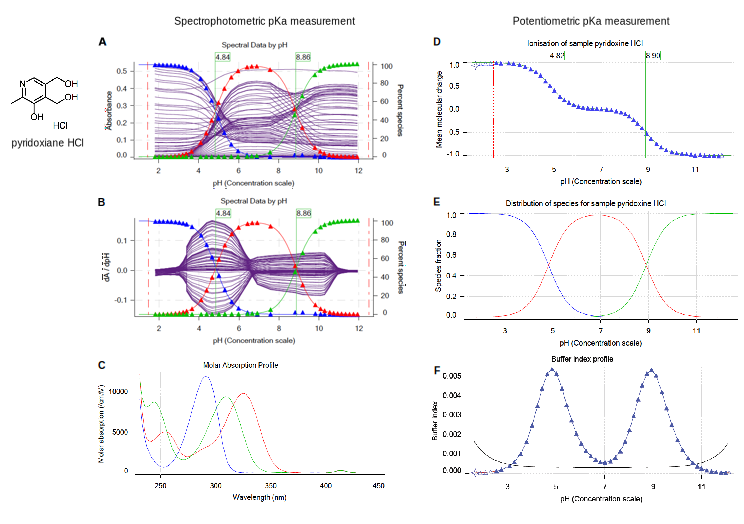
\includegraphics[width=0.95\linewidth]{figures/UVmetric_vs_pHmetric_pKa_figure}
\caption{{\bf Spectrophotometric (UV-metric) and potentiometric (pH-metric) pKa measurements of pyridoxine HCl with Sirius T3.} Spectrophotometic method (panels \textbf{A, B, C}) relies on UV-absorbance difference between protonation states.  It is very sensitive and requires very low analyte concentrations($\sim$ 50~\micro M), but limited to titration sites near chromophores. \textbf{A} Multiwavelength absorbance vs pH. Purple lines represents absorbance at each wavelength in UV-region.  \textbf{B} Derivative of multiwavelength absorbance with respect to pH (dA/dpH) vs pH is plotted with purple lines. In \textbf{A} and \textbf{B} Blue, red, and green triangles represent population of protonation states (from most protonated to least protonated) as calculated from experimental data at each pH value. pKa values (green flags) correspond to inflection point of multiwavelength absorbance data where change in absorbance with respect to pH is maximum. \textbf{C} Molar absorption coefficients vs wavelength for each protonation state as resolved by TFA. \textbf{D, E, F} illustrate potentiometric pKa measurement where molar addition of acid or base is tracked as pH is titrated.\textbf{D} Mean molecular charge vs pH. Mean molecular charge is calculated based on the model provided for the analyte: predicted number and nature of titratable sites(acid or base type), and number of counter ions present. pKa values are calculated as inflection points of charge vs pH plot. \textbf{E} Predicted macroscopic protonation state populations vs pH calculated based on pKa values (\ce{H2A+}: blue, \ce{HA}: red, and \ce{A-}: green) \textbf{E} Buffering index vs pH profile of water (grey solid line, theoretical) and the sample solution (blue triangles represent experimental data points). A higher concentration of analyte ($\sim$ 5~mM) is necessary for potentiometric method than for spectrophotometric method to provide large enough buffering capacity signal above water for an accurate measurement. 
}
\label{fig:UVmetric_vs_pHmetric_pKa}
\end{figure}

\todo[inline]{Brief outline of what this paper includes.}

%%%%%%%%%%%%%%%%%%%%%%%%%%%%%%%%%%%%%%%%%%%%%%%%%%%%%%%%%%%%
% Methods
%%%%%%%%%%%%%%%%%%%%%%%%%%%%%%%%%%%%%%%%%%%%%%%%%%%%%%%%%%%%
\section{Methods}

\subsection{Compound selection and procurement}
To select a set of small molecules focusing on chemical space representing kinase inhibitors for physicochemical property prediction challenges (pKa and lipophilicity) we started from kinase targeting subclass of ZINC15 chemical library ~\citep{sterling_zinc_2015} and applied a series of filtering and selection rules as depicted in Figure ~\ref{fig:compound_selection_figure} A. The following subsets of ZINC15 kinase subclass were selected in the first step: availability "now" and reactivity "anodyne", querried by:
\url{http://zinc15.docking.org/subclasses/kinase/substances/subsets/now+anodyne/}. "Now" label indicates availability of compound for immediate delivery. "Anodyne" label excludes compounds matching reactivity patterns and pan-assay interference compounds (PAINs) ~\citep{baell_new_2010, saubern_knime_2011}. 

Next, we found which these molecules were also found in eMolecules~\citep{eMolecules_ref_2017} (free version of the database was downloaded on June 1st, 2017), since procurement was going to be done through eMolecules. To find the intersection of ZINC15 kinase subset and eMolecules database, we matched molecules using canonical isomeric SMILES as identifier. Canonical isomeric SMILES were created with OpenEye OEChem Toolkit ~\citep{oechem_openeye_2017}. About 100~mg of each compound in powder form and 90\% purity was required complete planned experiments. To extract availability and price information from eMolecules, we queried using list of SMILES (as reported in eMolecules database) of the intersection set. We further filtered the intersection set of 1204 compounds based on delivery time (Tier 1 suppliers, 2 week delivery), at least 100 mg availability and in as powder (format: Supplier Standard Vial). 

pKa measurements and logP measurements with Sirius T3 requires a titratable group in the pKa range of 2-12, so we wanted to select compounds with predicted pKas in the range of 3-11 considering possible errors in pKa predictions. pKa predictions were calculated using Epik Sequential pKa prediction (scan)~\citep{shelley_epik:_2007,schrodinger_epik_v3_8} with target pH 7.0 and tautomerization allowed for generated states. We filtered out all compounds that did not have any pKas predicted between 3-11 and also compounds with predicted pKa values closer than 1 pKa unit so that individual pKas of multiprotic compounds could be resolved with spectrophotometric pKa measurements. With the goal of selecting compounds suitable for logP measurements, we eliminated compounds with OpenEye XlogP ~\citep{oemolprop_openeye_2017} values lower than -1 and higher than 6. 
Subsets of compounds with molecular weights between 150-350 g/mol and 350-500 g/mol were selected for fragment-like and drug-like categories respectively. We eliminated compounds which didn't have price and stock amounts information available. Also compounds with publicly available experimental logP measurements were removed. The sources we checked for experimental logP values were the following: DrugBank~\citep{wishart_drugbank:_2006} (queried with eMolecules SMILES), ChemSpider~\citep{pence_chemspider:_2010} (queried by canonical isomeric SMILES), NCI Open Database August 2006 release ~\citep{nci_open_database_2006} and Enhanced NCI Database Browser~\citep{nci_database_browser} (queried with canonical isomeric SMILES), and PubChem~\citep{kim_pubchem_2016} (queried with InChIKeys generated from canonical isomeric SMILES with NCI CACTUS Chemical Identifier Resolver~\citep{nci_chem_id_resolver}.)

In order to include common ring structures found in kinase inhibitors, we analyzed the frequency of rings found in FDA-approved kinase inhibitors via Bemis-Murcko fragmentation~\citep{bemis_properties_1996, oemedchemtk_openeye_2017}. Heterocycles found more than once in FDA-approved kinase inhibitors are shown in Figure \ref{fig:compound_selection_figure} B. 
While selection 25 compounds for fragment-like set and 10 compounds for drug-like set, We prioritized including at least one example of each heterocycle, although we failed to find compounds with piperazine and indazole that satisfied all other selection criteria. We observed that certain heterocycles (shown in Figure \ref{fig:compound_selection_figure} C) were overrepresented based on our selection criteria, thus limited the number of these structures in SAMPL6 challenge set to at most one in fragment-like and drug-like sets. To achieve broad and uniform sampling of logP dynamic range, we segregated the molecules into bins of logP values and selected compounds from each bin prioritizing cheaper chemicals. 

Presence of UV chromophores (absorbing in 200-400 nm) in proximity to protonation sites is necessary for spectrophotometric pKa measurements. To check for UV chromophores, we looked at the substructure matches to SMARTS pattern $[n,o,c][c,n,o]cc$ which were considered as the smallest unit of pi-conjugation that can constitute an UV-chromophore. This SMARTS pattern describes 4 heavy atom extended conjugation systems composed of aromatic carbon, nitrogen, or oxygen, such as 1.3-butadiene which absorbs at 217 nm. Additionally, final set of selected molecules were inspected to makes sure all potentially titratable groups were within 4 heavy atoms distance from a UV-chromophore.
25 fragment-like and 10 drug-like compounds were selected, out of which procurement and pKa measurements for 17(SM01-SM17) and 7(SM18-SM24) were successful, respectively. These 24 small molecules constituded the SAMPL6 pKa challenge set.

Python scripts used for compound selection are available at GitHub repository \href{https://github.com/choderalab/sampl6\textendash physicochemical\textendash properties}{https://github.com/choderalab/sampl6-physicochemical-properties} under \textbf{compound\textunderscore selection/ zinc15\textunderscore eMolecules\textunderscore intersection\textunderscore set} directory. Procurement details if each compound can be found in Table SI 1.

\begin{figure}
\begin{center}
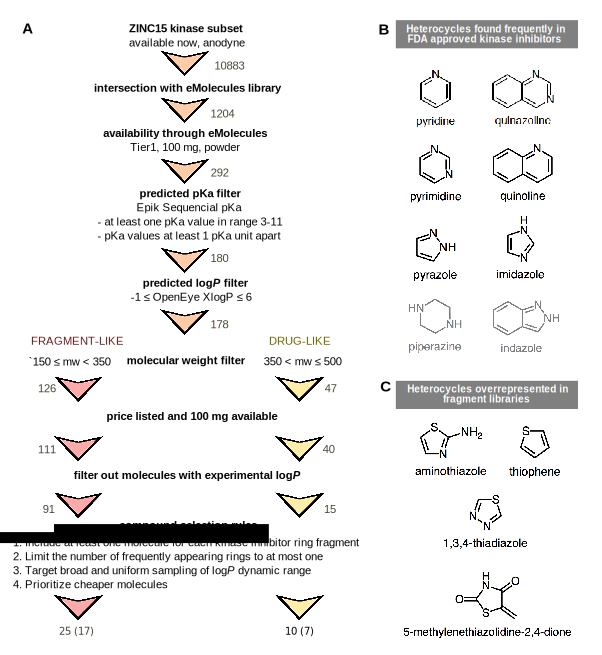
\includegraphics[width=0.95\linewidth]{figures/compound_selection_figure.pdf}
\caption{{\bf Compound selection for SAMPL6 physicochemical properties challenges for pKa and logP.} \textbf{A} Flowchart of filtering steps for the selection of SAMPL6 compounds similar to kinase inhibitors and kinase inhibitor fragments. Numbers next to arrows how number of potential compounds after each filtering step. 25 fragment-like and 10 drug-like compounds were selected, out of which procurement and pKa measurements for 17 and 7 were successful, respectively.   \textbf{B} Frequent heterocycles found in FDA approved kinase inhibitors determined by Bemis-Murcko fragmentation into rings  ~\citep{bemis_properties_1996}. Black structures were represented in SAMPL6 set at least once. Compounds with piperazine and indazole (gray structures) could not be included in the challenge set due to library and selection limitations.  \textbf{C} Structures of heterocycles that were overrepresented based on our compound selection workflow. We have limited occurance of these heterocycles to at most one.
}
\label{fig:compound_selection_figure}
\end{center}
\end{figure}




\subsection{UV-metric pKa measurements}

Experimental pKa measurements were collected using spectrophotometric pKa method with a Sirius T3 automated titrator instrument (Pion) at 25°C and constant ionic strength. Sirius T3 instrument is equiped with an Ag/AgCl double-junction reference electrode to monitor pH, a dip probe attached to spectrophotometer that measures, a stirrer, and automated volumetric titration capability. The UV-metric pKa measurement protocol of the Sirius T3 measures the change in multiwavelength absorbance in the 250-450 nm UV region of the absorbance spectrum while the pH is titrated between pH 1.8 and 12.2 to evaluate pKas~\citep{tam_multi-wavelength_2001, allen_multiwavelength_1998}. 

DMSO stock solutions of each compound with 10~mg/ml concentration were prepared by weighing 1 mg of powder chemical with Sartorius Analytical Balance (Model: ME235P) and dissolving it in 100~\micro L DMSO (Dimethyl sulfoxide, Fisher Bioreagents, CAT: BP231-100, LOT: 116070, purity $\geq$ 99.7\%).  DMSO stock solutions were capped immediately to limit hygroscopicity of DMSO and sonicated for 5-10 minutes in water bath sonicator at room temperature to ensure proper dissolution. These DMSO stock solutions were stored in room temperature up to 2 weeks. 10~mg/ml DMSO solutions were used as stock solutions for the preparation of 3 replicate samples for independent titrations:  1\-5 \micro L of 10~mg/ml DMSO stock solution delivered to 4~mL glass sample vials of Sirius T3 with an electronic micropipette (Rainin EDP3 LTS 1-10 \micro L). The volume of delivered DMSO stock solution, which determines the sample concentration, is optimized individually for each compound to achieve sufficient but not saturated absorbance signal (targeting 0.5-1.0 AU) in the linear response region. Another limiting factor for sample concentration was ensuring that the compounds stays soluble in the whole range of pH titration range. 25~\micro L of mid-range buffer (14.7~mM \ce{K2HPO4} 0.15 M \ce{KCl} in \ce{H2O}) was added to each sample transfered with a micropipette (Rainin EDP3 LTS 10-100 \micro L) to provide enough buffering capacity in middle pH ranges so that pH could be controlled incrementally throughout the titration.  

pH is temperature and ionic\textendash strength dependent. Sample heating block of Sirius T3 kept the analyte solution at $25 \pm 0.5$~\textdegree C throughout the titration. Ionic\textendash strength of the samples were adjusted by dilution in 1.5 mL ionic\textendash strength adjusted water (ISA water, 0.15~M KCl) to the vials by Sirius T3.  Analyte dilution, mixing, acid/base titration, and measurement of UV-absorbance was automated by UV-metric pKa measurement protocol of Sirius T3(Pion). pH was titrated between pH 1.8 and 12.2 with addition of acid (0.5~M HCl) and base (0.5~M KOH) targeting 0.2 pH steps between datapoints. Titrations were performed under Argon flow on the surface of sample solution to limit carbondioxide absorption from air. To capture all sources of experimental variability fully, instead of doing 3 tandem pH titrations on the same sample solution, pKas of three replicate samples were measured separately with one round of pH titration. Although this choice has higher cost for throughput and analyte consumption, it limits the dilution of the analyte during multiple titrations and drop in absorbance signal. 

Visual inspection of sample solutions after titration and inspection of pH-dependent absorbance shift in 500-600 nm region of UV spectra was used to verify no detectable precipitation occurred during the course of measurement. Absorbance in 500-600 nm region of UV spectra is associated with scattering of longer wavelengths of light in the presence of aggregates. For each analyte, we optimized analyte concentration, direction of titration and the range of pH titration in order to achieve solubility. The direction of titration was determined so that titration would start from the pH where the compound is most soluble: low-to-high pH for bases and high-to-low pH for acids. UV-metric pKa measurement method typically requires as low as 50~\micro M sample concentration (although minimum concentration requirement may change based on absorbance properties of the analyte). Some compounds may not be solube even at such low concentration throughout pH range of the titration. As the sample is titrated through a wide range of pH values, it is likely that low solubility ionization states such as neutral and zwitterionic states will be also be visited, limiting the highest analyte concentration that can be titrated without encountering any solubility issues.  For compounds with insufficient solubility to accurately determine a pKa directly in a UV-metric titration, a cosolvent protocol was used [See the next section: UV-metric pKa measurement with cosolvent]. 

Two Sirius T3 softwares, Sirius T3Control v1.1.3.0 and Sirius T3Refine v1.1.3.0, were used to execute measurement protocols and to analyze pH-dependent multivelenghth spectra, respectively.
A protonation state change of titratable sites near chromophores will modulate the UV-absorbance spectra of these chromophores, allowing populations of distinct UV-active species to be resolved as a function of pH. To do this, basis spectra are identified and populations extracted via TFA analysis of the pH-dependent multi-wavelength absorbance ~\citep{allen_multiwavelength_1998}. When fitting the absorbance data to a titratable molecule model to estimate pKas, we selected the minimum number of pKas that was sufficient to provide a high quality of fit between experimental and modeled data based on visual inspection of pH-dependent populations.

This method is capable of measuring pKas between 2 and 12 when protonatable groups are at most 4-5 heavy atoms away from chromophores such that a change in protonation state alters the absorbance spectrum of the chromophore. We have selected compounds where titratable groups are close to potential chromophores (generally aromatic ring systems), but it is possible that our experimental results couldn't detect protonation of titratable groups distal to a UV-chromophore.


\subsection{UV-metric pKa measurement with cosolvent}
If analytes are not sufficiently soluble in aqueous environment, pKa values can not be determined accurately with UV-metric pKa measurements method. If precipitation is present, the UV-absobance signal from pH-dependent precipitate formation can not be differentiated from the pH-dependent protonation signal. For compounds with low aqueous solubility pKa values were estimated from multiple apparent pKas measurements done in methanol:water cosolvent solutions with various ratios. This method is refered to as UV-metric psKa method in Sirius T3 Manual ~\citep{noauthor_sirius_2008}.

In cosolvent spectrophotometric pKa measurement protocol was very similar to UV-metric pKa measurement method in water except the following aspects: Three titrations were performed in typically in 30\%, 40\%, and 50\% mixtures methanol:water by volume to measure apparent pKa values (psKa) in these mixtures. Than Yasuda-Shedlovsky extrapolation method was used to estimate the pKa value at 0\% cosolvent~\citep{avdeef_ph-metric_1999,doi:10.1021/ac00049a010,TAKACSNOVAK1997235}. 

$$ psKa + log [\ce{H2O}]=A/\epsilon+B $$
Yasuda-Shedlovsky extrapolation relies on the linear correlation between $psKa + log [\ce{H2O}]$ and reciprocal dielectric constant of the cosolvent mixture ($1/\epsilon$). In the equation above, A and B are the slope and intercept of the line fitted to experimental datapoints.  Depending on the solubility requirements of the analyte methanol ratio of the cosolvent mixtures were adjusted. We designed the experiments to have at least 5\% cosolvent ratio difference between datapoints and 60\% methanol at most. Calculation of Yasuda-Shedlovsky extrapolation was performed by Sirius T3 software using at least 3 psKa values measured in different ratios of methanol:water.
Addition of methanol (ISA, 0.15 M KCl) was controlled by the instrument before each titration. Three consecutive pH titrations at different methanol concentrations were performed using the same sample solution. In addition, three replicate measurements with independent samples (prepared from the same DMSO stock) were collected.

\begin{figure}
\begin{center}
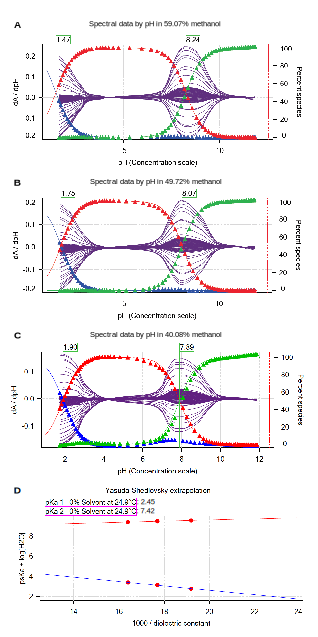
\includegraphics[width=0.5\linewidth]{figures/SM22_cosolvent_extrapolation_fig}
\caption{{\bf Determination of SM22 pKa values with cosolvent method and Yasuda-Shedlovsky extrapolation.} 
\textbf{A}, \textbf{B}, and \textbf{C} show psKa of SM22 determined at various methanol concentrations: 59.07\%, 49.72\%, 40.08\% by weight.  Purple solid lines indicate derivative of absorbance with respect to pH vs pH in multiple wavelength. psKa values (green flags) were determined by Sirius T3 Refinement Software. Blue, red and green triangles show relative populations of macroscopic protonation states with respect to pH calculated from the experimental data. Notice that as cosolvent concentration increases, psKa1 value decreases from 1.90 to 1.47 and psKa2 value increases from 7.84 to 8.24. \textbf{D} Yasuda-Shedlovsky extrapolation plot for SM22. Red datapoints correspond to psKa determined at various cosolvent ratios. Based on linear fitting to $psKa + log [\ce{H2O}]$ vs $1//\epsilon$, pKa1 and pKa2 in 0\% cosolvent (aqueous solution) was determined as 2.45 and 7.42, respectively. R\textsuperscript{2} values of linear fits are both 0.99. The slope of Yasuda-Shedlovsky extrapolation shows if the observed titration has acidic(positive slope) or basic(negative) character dominantly, although this is an macroscopic observation and should not be relied on for annotation of pKas to functional groups (microscopic pKas).
} 
\label{fig:YS_extrapolation}
\end{center}
\end{figure}

\subsection{Calculation of uncertainty in pKa measurements}
Experimental uncertainties were reported as standard error of the mean (SEM) of three replicate pKa measurements. Since Sirius T3 software reports pKa values with 2 decimal places, we have reported SEM as 0.01 in cases where SEM values calculated from 3 replicates were lower than 0.01.


\subsection{Protonation site determination with NMR}
\todo[inline]{Iyke will provide the text for NMR method.}

\subsection{Quality control for chemicals}
Purity of SAMPL6 pKa challenge compounds were determined based on LC\textendash MS. The purity analysis was performed using an Agilent HPLC1200 Series equipped with auto\textendash  sampler, UV diode array detector and a Quadrupole MS detector 6140. The software used was Chemistation for LC \& LC\/MS with version C01.07SR2.
The column for the analysis is Assentis Express C18 3.0x100mm 2.7~µl particle size at Column temperature~=~45\textdegree C.
\begin{itemize}

\item Mobile phase A: 2~mM ammonium formate ( pH=3.5) aqueous
\item Mobile phase B: 2~mM ammonium formate in Acetonitrile : Water=90:10 ( pH=3.5)
\item Flow rate : 0.75ml/min
\item Gradient: Starting with 10\% B to 95\%B in 10 minutes then hold 95\%B for 5 minutes. 
\item Post run length: 5 minutes 
\item Mass condition: ESI positive and negative mode
\item Capillary voltage: 3000~V
\item Grying gas flow: 12~ml/min
\item Nebulizer pressure: 35~psi
\item Drying temperature: 350\textdegree C
\item Mass range: 5-1350~Da; Fragmentor:70; Threshold:100
\end{itemize}

The percent area for main peak is calculated based on the area of main peak divided by the total area of all peaks. The percent area of the main peak is reported as an estimate of sample purity.

%%%%%%%%%%%%%%%%%%%%%%%%%%%%%%%%%%%%%%%%%%%%%%%%%%%%%%%%%%%%
% Results
%%%%%%%%%%%%%%%%%%%%%%%%%%%%%%%%%%%%%%%%%%%%%%%%%%%%%%%%%%%%
\section{Results}

\subsection{Spectrophotometric pKa measurements}
todo[inline]{Summarize measurement results, refer to tables and SI.}

\begin{figure}
\includegraphics[width=0.95\linewidth]{figures/SAMPL6_pKa_molecules_fig}
\caption{{\bf Molecules used in the SAMPL6 \pKa  challenge.} 
Experimental UV-metric \pKa measurements were performed for these 24 molecules, and discernable macroscopic {\pKa}s reported. 
Uncertainties are expressed as the standard error of the mean (SEM) of three independent measurements. Structure figures were created with OpenEye OEDepict Toolkit ~\citep{oedepict_openeye_2017}
}
\label{fig:pKa_molecules}
\end{figure}


\begin{table}[tb!]
\begin{center}
\begin{threeparttable}
\centering
\caption{{\bf Experimental pKas of SAMPL6 compounds.} Spectrophotometric pKa measurements were performed with two assay types based on aqueous solubility of analytes. "UV-metric pKa" assay indicates spectrophotometric pKa measurements done with Sirius T3 in ISA water. "UV-metric pKa with cosolvent" assay refers to pKa determination by Yasuda-Shedlovsky extrapolation from psKa measurements in various ratios of ISA methanol:water mixtures. Triplicate measurements were performed at $25 \pm 0.5$~\textdegree C and in the presence of approximately 150 mM \ce{KCl} to adjust ionic strength.} 
\label{my-label}
\begin{tabular}{@{}lllll@{}}
\toprule
Molecule ID & pKa\textsubscript{1} & pKa\textsubscript{2} & pKa\textsubscript{3} & Assay Type \\ \midrule
SM01 & 9.53 $\pm$ 0.01 &  &  & UV-metric pKa \\
SM02 & 5.03 $\pm$ 0.01 &  &  & UV-metric pKa with cosolvent \\
SM03 & 7.02 $\pm$ 0.01 &  &  & UV-metric pKa with cosolvent \\
SM04 & 6.02 $\pm$ 0.01 &  &  & UV-metric pKa \\
SM05 & 4.59 $\pm$ 0.01 &  &  & UV-metric pKa with cosolvent \\
SM06 & 3.03 $\pm$ 0.04 & 11.74 $\pm$ 0.01 &  & UV-metric pKa \\
SM07 & 6.08 $\pm$ 0.01 &  &  & UV-metric pKa \\
SM08 & 4.22 $\pm$ 0.01 &  &  & UV-metric pKa \\
SM09 & 5.37 $\pm$ 0.01 &  &  & UV-metric pKa with cosolvent \\
SM10 & 9.02 $\pm$ 0.01 &  &  & UV-metric pKa with cosolvent \\
SM11 & 3.89 $\pm$ 0.01 &  &  & UV-metric pKa \\
SM12 & 5.28 $\pm$ 0.01 &  &  & UV-metric pKa \\
SM13 & 5.77 $\pm$ 0.01 &  &  & UV-metric pKa \\
SM14 & 2.58 $\pm$ 0.01 & 5.30 $\pm$ 0.01 &  & UV-metric pKa \\
SM15 & 4.70 $\pm$ 0.01 & 8.94 $\pm$ 0.01 &  & UV-metric pKa \\
SM16 & 5.37 $\pm$ 0.01 & 10.65 $\pm$ 0.01 &  & UV-metric pKa \\
SM17 & 3.16 $\pm$ 0.01 &  &  & UV-metric pKa \\
SM18 & 2.15 $\pm$ 0.02 & 9.58 $\pm$ 0.03 & 11.02 $\pm$ 0.04 & UV-metric pKa with cosolvent \\
SM19 & 9.56 $\pm$ 0.02 &  &  & UV-metric pKa with cosolvent \\
SM20 & 5.70 $\pm$ 0.03 &  &  & UV-metric pKa with cosolvent \\
SM21 & 4.10 $\pm$ 0.01 &  &  & UV-metric pKa with cosolvent \\
SM22 & 2.40 $\pm$ 0.02 & 7.43 $\pm$ 0.01 &  & UV-metric pKa with cosolvent \\
SM23 & 5.45 $\pm$ 0.01 &  &  & UV-metric pKa with cosolvent \\
SM24 & 2.60 $\pm$ 0.01 &  &  & UV-metric pKa with cosolvent \\ \bottomrule
\end{tabular}
\begin{tablenotes}
\item[1] pKa values are reported as mean and SEM of three replicates.
\end{tablenotes}
\end{threeparttable}
\end{center}
\end{table}

\subsection{Impact of cosolvent to UV-metric pKa measurements}
For molecules with insufficient solubility in aqueous medium throughout the titration range (pH 2-12), we had to use UV-metric pKa measurement with cosolvent methanol. To confirm that UV-metric pKa measurements with cosolvent method lead to indistinguishable results compared to UV-metric measurements in water, we collected pKa values of 12 highly soluble SAMPL6 compounds and pyridoxine also with cosolvent method. Correlation analysis of pKa values measured with two methods show that using methanol as cosolvent and determining aqueous pKas via Yasuda-Shedlovsky extrapolation did not cause any bias (Figure ~\ref{fig:water_vs_cosolvent_pKa_correlation}). 

\begin{figure}
\begin{center}
\includegraphics[width=0.5\linewidth]{figures/water_vs_cosolvent_pKa_values_correlation_figure.pdf}
\caption{{\bf pKa measurements with UV-metric method with cosolvent and UV-metric method in water show good correlation.} 
17 pKa values(blue marks) of 13 chemicals were measured with both UV-metric pKa method in water and UV-metric pKa method with methanol as cosolvent (Yasuda-Shedlovsky extrapolation to 0\% methanol). Dashed black line has slope of 1, representing perfect correlation.  Dark and light green shaded areas indicate +-0.5 and +-1.0 pKa unit difference regions, respectively. Error bars are plotted as SEM of replicate measurements, although they are not visible since the largest SEM value is 0.04. MD: Mean difference, MAD: Mean absolute deviation, RMSD: Root-mean-square deviation.  
}
\label{fig:water_vs_cosolvent_pKa_correlation}
\end{center}
\end{figure}

\subsection{Purity of SAMPL6 compounds}
\todo[inline]{summarize results of LC-MS measurements}
LC-MS based purity measurements showed that powder stocks of 23 SAMPL6 pKa challenge compounds were >90\% pure and purity of SM22 was 87\% which was the lowest in the set (Table SI 6).  Additionally, molecular weights detected by LC-MS method were consistent with molecular weights reported in eMolecules and supplier reported molecular weights when provided. 
\subsection{Characterization of SM07 microstates with NMR}
\todo[inline]{Add results of NMR analysis of SM07 - from Iyke}


%%%%%%%%%%%%%%%%%%%%%%%%%%%%%%%%%%%%%%%%%%%%%%%%%%%%%%%%%%%%
% Discussion
%%%%%%%%%%%%%%%%%%%%%%%%%%%%%%%%%%%%%%%%%%%%%%%%%%%%%%%%%%%%
\section{Discussion}
\todo[inline]{Discussion of experimental data interpretation: macroscopic}
Multiwavelength absorbance analysis on thw Sirius T3 allows for very good resolution of pKas, but it is important to note that this method produces estimates of macroscopic pKas. If multiple microscopic pKas have close pKa values and overlapping changes in UV absorbance spectra associated with protonation/deprotonaton event, the spectral analysis could produce a single macroscopic pKa that represents an aggregation of multiple microscopic pKas.
\todo[inline]{Warning about acid base assingment from cosolvent measurements}
\todo[inline]{Lessons learned for future challenge iterations}
\todo[inline]{Discussion of NMR results}
The goal of this NMR characterization was collecting information on microscopic states related to experimental pKa measurements, i.e. determining sites of protonation. pKa measurements performed with spectrophotometric method provides macroscopic pKa values, but does not provide information site of protonation. On the other hand, most computational prediction methods predict primarily microscopic pKa values. Protonation sites can be determined by NMR methods, although these measurements are very laborious in terms of data collection and interpretation compared to pKa measurements with Sirius T3. Moreover, not all SAMPL6 molecules were suitable for NMR measurements due to high sample concentration requirements (for methods other than proton NMR) and analyte solubility issues. Thus we performed NMR based microstate characterization only for SM07. We investigated microstates existed at pH values lower and higher than macroscopic pKa value with the goal of evaluating if spectroscopicly measured pKa was microscopic (related to single protonation site).
\todo[inline]{Interpretation of NMR microstates for 4-amino quinazoline series }
In addition to SM07, there were 5 other 4-amino quinazoline derivatives in SAMPL6 set: SM02, SM04. SM09, SM12, and SM13. Based on structural similarity, we can infer that spectrometric pKa values measured for other 4-amino quinazoline compounds as microscopic pKa related to the protonation of the same quinazoline nitrogen with the same neutral background protonation states.
\todo[inline]{Challenges with NMR measurments?}
\todo[inline]{pKa can shift based on ionic strength, temperature, and lipophilic content
Can other cosolvents be interesting for process chemistry.}

%%%%%%%%%%%%%%%%%%%%%%%%%%%%%%%%%%%%%%%%%%%%%%%%%%%%%%%%%%%%
% Code and Data Availability
%%%%%%%%%%%%%%%%%%%%%%%%%%%%%%%%%%%%%%%%%%%%%%%%%%%%%%%%%%%%
\section{Code and data availability}
\begin{minipage}{15cm}
\begin{itemize}
%\item Compound selection scripts are available at \href{https://github.com/}{https://github.com/} under \"compound_selection\" directory.
% https://github.com/choderalab/sampl6-physicochemical-properties

\item SAMPL6 pKa challenge instructions, submissions, and analysis is available at  \href{https://github.com/MobleyLab/SAMPL6}{https://github.com/MobleyLab/SAMPL6}

\item Python scripts used for compound selection are available at \textbf{compound\textunderscore selection} directory of  
\href{https://github.com/choderalab/sampl6\textendash physicochemical\textendash properties}{https://github.com/choderalab/sampl6-physicochemical-properties}

\end{itemize}
\end{minipage}



\todo[inline]{Construct a proper README for compound selection directory.}
%%%%%%%%%%%%%%%%%%%%%%%%%%%%%%%%%%%%%%%%%%%%%%%%%%%%%%%%%%%%
% Overview of supplementary information
%%%%%%%%%%%%%%%%%%%%%%%%%%%%%%%%%%%%%%%%%%%%%%%%%%%%%%%%%%%%
\section{Overview of supplementary information}

Organized in SI document:

- TABLE SI 1: procurement details of SAMPL6 compounds  
% procurement_details_of_SAMPL6_compounds.csv 

- TABLE SI 2: selection details of SAMPL6 compounds  
% selection_details_of_SAMPL6_compounds.csv 

- TABLE SI 3: pKa results of replicate experiments csv
% pKa_results_of_replicate_experiments.csv

- TABLE SI 4: pKa results of water and cosolvent replicate experiments csv
% water_vs_cosolvent_pKa_values_including_pyridoxineHCl.csv

- TABLE SI 5: pKa mean and SEM results of water and cosolvent replicate experiments
% statistics_of_UV-metric_pKa_measurements_in_water_vs_cosolvent.csv  
% pKas without SEM reported has 1 replicate
% pKas with SEM values calculated were performed in triplicates

- NMR spectra of SM07 microstate characterization  

- TABLE SI 6: Summary of LC-MS purity results
% purity_of_SAMPL6_pKa_compounds_determined_by_LCMS.csv


- LC-MS Figures  


Extra files:  

- Sirius T3 reports  



%%%%%%%%%%%%%%%%%%%%%%%%%%%%%%%%%%%%%%%%%%%%%%%%%%%%%%%%%%%%
% Author Contributions 
%%%%%%%%%%%%%%%%%%%%%%%%%%%%%%%%%%%%%%%%%%%%%%%%%%%%%%%%%%%%
\section{Author Contributions}
\todo[inline]{Complete this section.}

Conceptualization, ; Methodology, ; Software, ; Formal Analysis, ; Investigation, MI, ; Resources, ;  Data Curation, ; Writing-Original Draft, ; Writing - Review and Editing, ; Visualization, ; Supervision, ; Project Administration, ; Funding Acquisition, 

%(Follow the \href{http://www.cell.com/pb/assets/raw/shared/guidelines/CRediT-taxonomy.pdf}{CRediT Taxonomy})

%%%%%%%%%%%%%%%%%%%%%%%%%%%%%%%%%%%%%%%%%%%%%%%%%%%%%%%%%%%%
% Acknowledgments 
%%%%%%%%%%%%%%%%%%%%%%%%%%%%%%%%%%%%%%%%%%%%%%%%%%%%%%%%%%%%
\section{Acknowledgments}
\todo[inline]{Complete this section.}

MI, ASR, and JDC acknowledge support from the Sloan Kettering Institute. JDC acknowledges support from NIH grant P30 CA008748. MI acknowledges Doris J. Hutchinson Fellowship. Acknowledging Merck Preformulation department for materials, expertise and instrument time.

Brad Sherborne  
Paul Czodrowski - helped with purchasable compound list in earlier iteration  
Ikenna Ndukwe  
Caitlin Bannan  

%%%%%%%%%%%%%%%%%%%%%%%%%%%%%%%%%%%%%%%%%%%%%%%%%%%%%%%%%%%%
% Disclosures 
%%%%%%%%%%%%%%%%%%%%%%%%%%%%%%%%%%%%%%%%%%%%%%%%%%%%%%%%%%%%
\section{Disclosures}

JDC is a member of the Scientific Advisory Board for Schr\"{o}dinger, LLC.

\nocite{*} % This command displays all refs in the bib file. PLEASE DELETE IT BEFORE YOU SUBMIT YOUR MANUSCRIPT!
\bibliography{elife-sample}

%%%%%%%%%%%%%%%%%%%%%%%%%%%%%%%%%%%%%%%%%%%%%%%%%%%%%%%%%%%%
% Supplementary Information
%%%%%%%%%%%%%%%%%%%%%%%%%%%%%%%%%%%%%%%%%%%%%%%%%%%%%%%%%%%%
%\newpage
%\section{Supplementary Information}






\end{document}
